\chapter{Diseño del sistema}
\label{cap:diseno}
El diseño articula los requerimientos del capítulo~\ref{cap:requerimientos}
con las responsabilidades y los datos del prototipo. Las vistas siguientes
reconstruyen la organización existente y distinguen las extensiones propuestas.
Los detalles de procesamiento y los registros por incremento se desarrollan
en el capítulo~\ref{cap:implementacion}.

\section{Arquitectura}
\label{sec:arquitectura-neuma}
La aplicación está organizada en un único módulo Android, \texttt{:app}, con
paquetes por actividad y servicios compartidos. La separación es de
responsabilidades dentro del mismo proceso. Las pantallas Compose presentan
estado y reciben acciones; los ViewModels coordinan esas acciones, las operaciones
asíncronas y el ciclo de vida. Las sesiones concentran las reglas musicales,
la evaluación y las transiciones propias de cada juego.

Las sesiones de instrumentos, ritmo, Defender y voz conservan modelos distintos.
Comparten criterios e infraestructura donde corresponde, sin imponer una clase
genérica de juego. En particular, el motor Mamdani recibe configuraciones y
entradas; cada actividad decide cómo obtener sus indicadores, interpretar la
salida y aplicar límites. Esta distribución permite revisar la matemática común
y las políticas particulares por separado, de acuerdo con RF-09 y RF-15.

Los servicios de captura, reproducción y resultados se conectan mediante
interfaces o dependencias suministradas por constructor. \texttt{MainActivity}
reúne las instancias Android, los repositorios de archivos y los ViewModels,
y coordina navegación y notificaciones de ciclo de vida. En el recorrido vocal,
la coordinación separa reproducción de referencia, captura y cierre: el núcleo
recibe estimaciones y tiempos, sin administrar el micrófono.

La figura~\ref{fig:arquitectura-neuma} sintetiza estas colaboraciones. Rhythm Tap
integra una WebView local para representar la partitura y su estado. Generación,
taps, reloj y evaluación permanecen en Kotlin, con recursos de grabado incluidos
en la aplicación.

\begin{figure}[p]
  \centering
  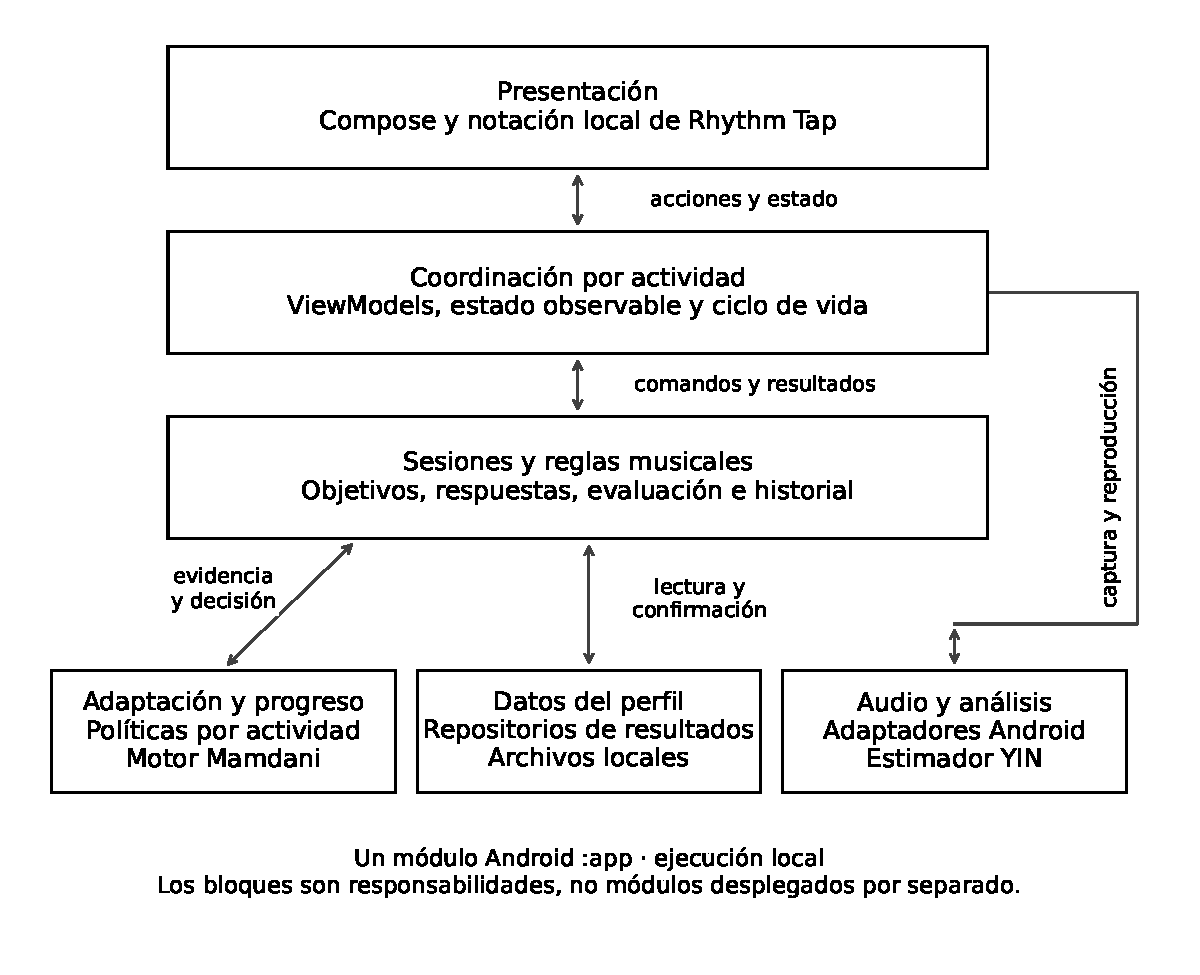
\includegraphics[width=\textwidth]{figuras/arquitectura-neuma.pdf}
  \caption{Responsabilidades y colaboraciones de la arquitectura implementada.
  Los bloques pertenecen al mismo módulo y no indican servicios remotos.}
  \label{fig:arquitectura-neuma}
\end{figure}
\clearpage

\section{Modelo de dominio}
\label{sec:modelo-dominio}
El modelo de la figura~\ref{fig:dominio-neuma} relaciona actividad, partida,
ronda, respuesta, resultado, decisión y progreso. Utilizo el vocabulario de
\path{CONTEXT.md}; la figura expresa conceptos y no tablas o clases obligatorias.
La configuración de práctica identifica contenido, modo, ayuda y exigencia,
necesarios para interpretar el resultado.

La relación entre partida y ronda depende de la actividad. Instrumentos agrupa
preguntas; la progresión vocal, rondas de un intervalo y ayuda determinados.
En Rhythm Tap una partida es un único ejercicio. Defender evalúa intentos sobre
objetivos simultáneos hasta el cierre de la partida. El modelo admite resultados
del ejercicio y del conjunto, sin convertir todos esos recorridos en la misma
secuencia de rondas.

La respuesta musical y su evaluación son conceptos diferentes: una respuesta
estable puede ser incorrecta y una señal insuficiente puede dejar el ejercicio
sin completar. A su vez, el resultado musical, la confirmación de su guardado
y su aptitud para acreditar progreso son condiciones distintas. Esta separación
evita equiparar completar una acción con dominar un contenido.

El progreso se interpreta por habilidad y condiciones de práctica. En voz se
distinguen intervalo, dirección y ayuda; en ritmo, categoría y tempo; en Defender,
variante y contenido. Una mejora en una de esas condiciones no transfiere
automáticamente evidencia a las demás. El perfil local reúne los resultados
y el progreso, sin representar una cuenta o una identidad remota.

\begin{figure}[p]
  \centering
  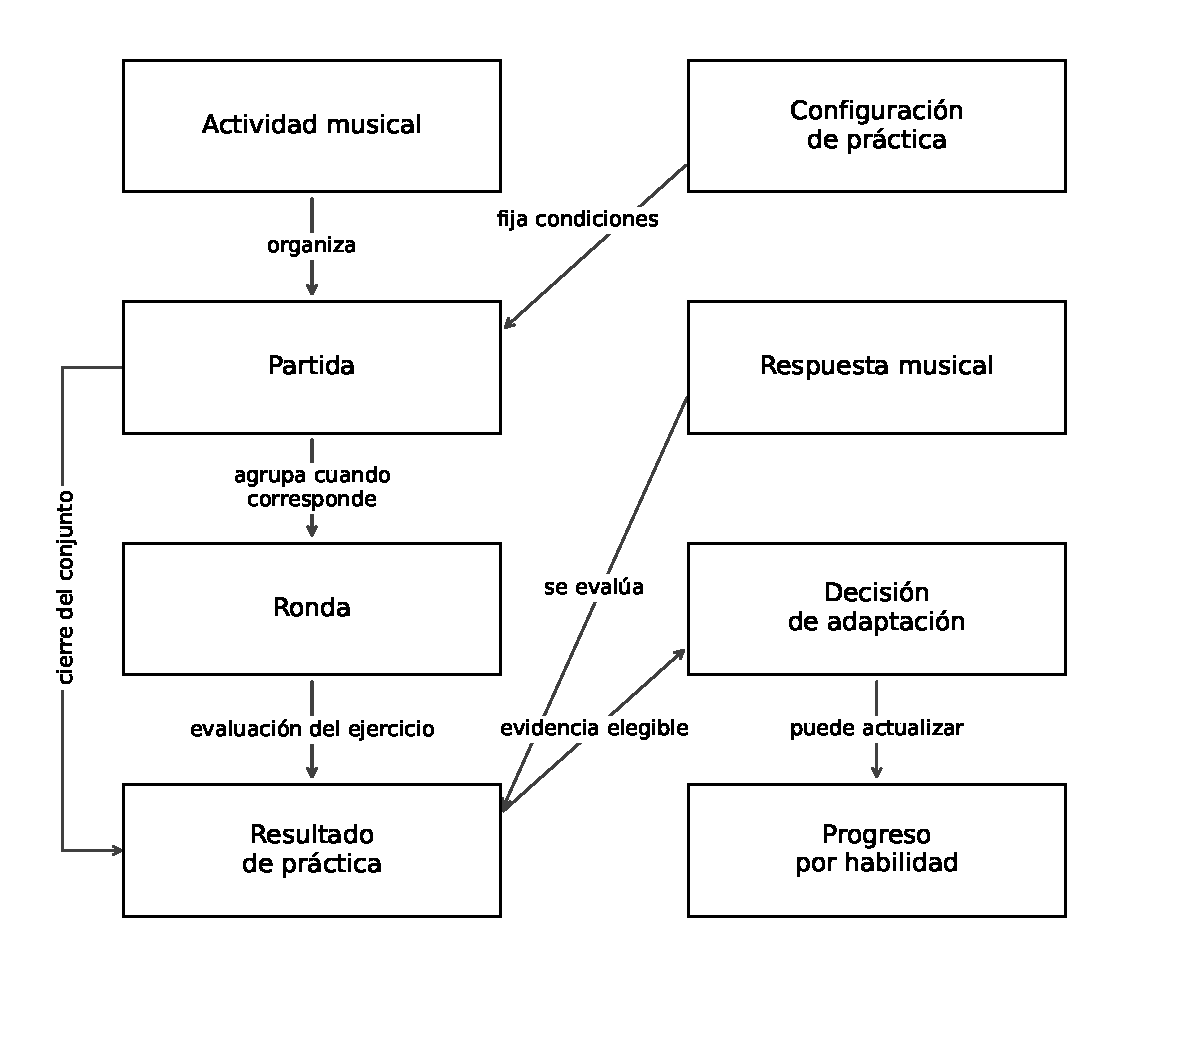
\includegraphics[width=\textwidth]{figuras/dominio-neuma.pdf}
  \caption{Modelo conceptual de la práctica y adaptación. Las relaciones resumen
  responsabilidades comunes; su granularidad se concreta por actividad.}
  \label{fig:dominio-neuma}
\end{figure}
\clearpage

\section{Criterios de práctica, ayudas y progresión}
\label{sec:diseno-practica}
Los criterios siguientes reúnen las decisiones de diseño y propuestas funcionales
que adopté para el proyecto y registré en las guías de trabajo. Orientan el diseño y no
implican que todas las funciones estén implementadas o evaluadas.

La práctica prioriza la superación personal, el avance por habilidad y el acceso
a nuevos desafíos. Las recompensas visuales son un complemento posible sin un
sistema concreto definido. Busco permitir reintentos conservando el progreso
ya conseguido; vidas y límites temporales se revisan según cada actividad. El
sistema orienta y recomienda, manteniendo elección de habilidades y repaso de
contenidos disponibles. Recomendar y desbloquear cumplen funciones distintas.

La propuesta de continuidad utiliza una meta semanal de días de práctica como
referencia principal y una racha diaria opcional como apoyo secundario. Los días
de actividad se registran separadamente de resultados musicales e hitos; una
interrupción de asistencia no equivale a pérdida de una habilidad. La comparación
con otras formas de organizar la práctica permanece abierta.

Las ayudas deben identificar qué parte de la tarea resuelven. Escuchar dos notas,
recibir solo un ancla o producir ambas sin referencia plantea condiciones distintas.
La propuesta de ofrecer una melodía conocida después de un error exige verificar
intervalo, dirección y familiaridad del repertorio, conservando el canto como
respuesta. El antecedente de la sección~\ref{sec:aprendizaje-practica} no evalúa
esa intervención posterior al error ni la extiende a todos los intervalos.

La lectura rítmica permite inspeccionar la partitura antes de iniciar, sin escuchar
previamente un modelo de la solución. El primer intento y las repeticiones del mismo
patrón deben diferenciarse. El dictado por selección de partitura con reescuchas y
la escucha de conjuntos son propuestas futuras. Esta última requiere grabaciones
que aportaré y anotaré, selección dentro de tramos aptos e identificación
de instrumentos y funciones en pasos separados. Su progresión deberá distinguir
ambos desempeños; no incorpora extracción automática de pistas.

\section{Modelo de ajuste difuso y aplicación de decisiones}
\label{sec:diseno-dda}
El esquema siguiente explicita los operadores del motor y los criterios para
aplicar su salida. Las funciones de pertenencia, indicadores, límites y reglas
concretas se configuran por actividad; sus valores siguen siendo experimentales.
La pertenencia se representa mediante
\begin{equation}
  \mu_A\colon X\longrightarrow[0,1].
  \label{eq:pertenencia-difusa}
\end{equation}
Definir un término como desempeño alto requiere fijar su dominio, forma y
solapamiento con los demás términos. Una proporción de aciertos, un tiempo de
respuesta y un error de afinación tienen interpretaciones distintas y no se
intercambian sin atender a la tarea.

\subsection{Operadores de inferencia y desfusificación}
\label{sec:inferencia-mamdani}
En un sistema Mamdani, cada regla produce un conjunto difuso de salida. El proceso
comprende la evaluación de pertenencias de entrada, la combinación de condiciones,
la implicación y la agregación de las consecuencias
\parencite{mathworksProcesoDifuso}. Para expresar el esquema mínimo--máximo,
considérese una regla de peso unitario: si \(x_1\) pertenece a \(A_1\) y \(x_2\)
pertenece a \(A_2\), entonces la salida pertenece a \(B_r\). Su activación es
\begin{equation}
  \alpha_r=\min\bigl(\mu_{A_1}(x_1),\mu_{A_2}(x_2)\bigr).
  \label{eq:activacion-mamdani}
\end{equation}
La implicación por mínimo recorta la pertenencia del consecuente a esa activación.
La agregación por máximo reúne las salidas de las \(R\) reglas:
\begin{equation}
  \mu_{\mathrm{salida}}(y)=
  \max_{1\leq r\leq R}\min\bigl(\alpha_r,\mu_{B_r}(y)\bigr).
  \label{eq:agregacion-mamdani}
\end{equation}
Estos operadores constituyen una configuración concreta; existen otras opciones
de combinación e implicación \parencite{mathworksProcesoDifuso}.

Como ejemplo conceptual del proyecto, una regla podría relacionar aciertos altos
y respuesta rápida con un aumento de dificultad. Su utilidad depende de que ambos
indicadores sean pertinentes para esa actividad: responder más rápido no siempre
representa una ejecución musical mejor. El ejemplo ilustra la estructura de una
regla y no fija una condición nueva para los juegos implementados. La base concreta
de reglas debe documentarse junto con sus entradas y consecuencias para permitir
revisar qué criterio expresa cada decisión.


\label{sec:centroide-ajuste}
La agregación produce una función de pertenencia, mientras que el juego necesita
una decisión ejecutable. La desfusificación convierte esa salida en un valor
numérico. El método del centroide calcula su centro de gravedad; en una
representación discreta combina las posiciones evaluadas con sus pertenencias
\parencite{mathworksDesfusificacion}. Si se aproxima mediante integración
trapezoidal sobre puntos equidistantes \(y_0,\ldots,y_N\), puede escribirse como
\begin{equation}
  y^* =
  \frac{\sum_{i=0}^{N}w_i\,y_i\,\mu_{\mathrm{salida}}(y_i)}
       {\sum_{i=0}^{N}w_i\,\mu_{\mathrm{salida}}(y_i)},
  \qquad
  w_0=w_N=\frac{1}{2},\quad w_i=1\ (0<i<N).
  \label{eq:centroide-discreto}
\end{equation}
El paso constante de la discretización se cancela en el cociente. Esta expresión
requiere un denominador positivo. Si ninguna regla aporta pertenencia en los puntos
evaluados, no proporciona un centroide válido. El comportamiento ante esa condición
debe establecerse explícitamente en el diseño del motor.

En Neuma interesa separar el resultado de la inferencia de la modificación que
finalmente se aplica. Una salida numérica puede transformarse en una propuesta de
aumento, mantenimiento o reducción; después intervienen los límites y las reglas
de la actividad. Por ejemplo, una propuesta de aumentar la exigencia puede no
producir cambios si ya se alcanzó el máximo permitido. Registrar ambos resultados
permite explicar esa diferencia y reconstruir la decisión.

La especificación debe identificar el intervalo de salida, la cantidad de puntos
y el tratamiento de entradas ausentes o inválidas. Las pruebas del cálculo
comprueban su ejecución; evaluar el DDA exige examinar además la pertinencia
del ajuste para la habilidad que se practica.


\subsection{Aplicación y progresión}
\label{sec:adaptacion-progresion}
La adaptación del desafío y la progresión de contenidos operan sobre decisiones
diferentes. En el diseño del proyecto, el DDA puede modificar condiciones dentro
de una partida o entre ejercicios, según la actividad. El desbloqueo determina
cuándo se habilitan otros contenidos a partir del desempeño acumulado. Una
reducción transitoria de dificultad y la conservación de un contenido habilitado
pueden coexistir; sus reglas deben describirse por separado.

Modificar una consigna ya presentada puede alterar las condiciones iniciales del
intento. Cada actividad necesita definir qué elementos permanecen fijados, cuáles
pueden adaptarse y cuándo se hace efectivo un cambio. Este criterio permite revisar
la coherencia de reglas y devoluciones señalada en la sección~\ref{sec:desafio-dda}.

Para estudiar la conducta del motor se requiere conservar la relación entre los
datos observados y la decisión: actividad y contenido, dificultad y ayudas,
indicadores utilizados, configuración de pertenencias y reglas, salida inferida
y ajuste aplicado. La ventana de observación y las restricciones entre cambios
también deben identificarse cuando formen parte del diseño. Esta trazabilidad
permite distinguir una decisión calculada por el motor de una intervención manual
o de la ausencia de información suficiente para ajustar.

La elección de lógica difusa organiza una política explícita de adaptación, pero
no demuestra que esa política sea óptima. Su justificación para Neuma reside en
poder expresar y revisar los criterios que relacionan observaciones con ajustes.
Determinar si esos ajustes sostienen un desafío abordable requiere evaluación
con participantes; establecer retención o transferencia exige las comprobaciones
descritas en la sección~\ref{sec:desempeno-aprendizaje}. Las simulaciones y las
pruebas de software aportan evidencia sobre la ejecución de la política y deben
mantenerse diferenciadas de esas preguntas pedagógicas.


\section{Diseño de datos}
\label{sec:diseno-datos}
La persistencia utiliza documentos JSON por actividad y configuraciones del
perfil. Cada tipo conserva la estructura necesaria para su tarea: respuestas
y escuchas en instrumentos, partitura y ataques en ritmo, objetivos e intentos
en Defender, y mediciones derivadas y referencias en voz. Los identificadores,
versiones y campos de procedencia permiten relacionar esos datos con el contexto
de ejecución; no se almacena una grabación de la voz.

Los repositorios de resultados ocultan el acceso a archivos detrás de operaciones
de lectura y guardado. La escritura prepara un documento temporal y procura
reemplazar el anterior mediante movimiento atómico; si el sistema de archivos
no admite esa operación, utiliza reemplazo ordinario. Por tanto, la estrategia
reduce escrituras parciales, sin constituir una garantía absoluta de durabilidad.
Las operaciones se serializan mediante una exclusión compartida por directorio
de perfil para coordinar guardado, exportación y reinicio.

En ritmo, Defender y voz, la preparación del resultado reúne las decisiones y
los estados de progreso bajo la misma coordinación que su persistencia. Los
reintentos conservan identidad y, cuando corresponde, revisión, evitando duplicar
el avance. El progreso se reconstruye desde los registros confirmados y sus
estados asociados. Un resultado pendiente se mantiene identificado en memoria;
no se promete conservarlo si el proceso termina antes de guardarlo o exportarlo.
Estas decisiones atienden RF-11 y RNF-02.

La exportación JSON ofrece una vista interpretada con configuración, progreso
y procedencia. La copia ZIP conserva los archivos originales, incluso si alguno
está dañado o es incompatible, y puede incluir pendientes: es un recurso de
recuperación para análisis externo, sin importación o reparación automática.
El reinicio utiliza un marcador para completar un borrado interrumpido al próximo
inicio e invalida operaciones anteriores; los archivos ya exportados permanecen
fuera de ese borrado. Estos recorridos corresponden a RF-13 y RF-14.

\section{Patrones utilizados}
\label{sec:patrones-diseno}
El diseño utiliza ViewModel con estado observable para separar la coordinación
de la representación. Las pantallas observan ese estado y envían acciones;
las sesiones no necesitan conocer cómo se dibuja una nota o se organiza una
pantalla. La separación permite comprobar acciones y resultados con tiempo,
azar, audio y almacenamiento controlados, conforme al método de verificación
de la sección~\ref{sec:metodo-evaluacion}.

El acceso a resultados sigue la función de un repositorio: las sesiones trabajan
contra contratos específicos y existen implementaciones de archivos o memoria.
Los adaptadores de audio conectan esos contratos con Android. Las dependencias
se suministran por constructor o funciones, sin un contenedor de inyección.
La composición manual permite sustituir recursos en pruebas y escenarios
simulados sin escribir en el perfil real.

Las fases explícitas de las sesiones organizan transiciones válidas y estados
terminales. Por ejemplo, la ronda vocal distingue espera del ancla, captura,
espera del objetivo, evaluación completa e interrupción. No requiere una jerarquía
de objetos de estado: la sesión procesa acciones y expone su estado. Los
temporizadores y las respuestas tardías deben respetar esos cierres.

\section{Extensiones de diseño pendientes}
La respuesta en piano de Defender deberá integrarse con contenido, audio,
historial y progreso propios de la variante, manteniendo la evaluación del
conjunto exacto de teclas con octavas exigida por RF-07. La gobernanza automática
de ayuda vocal de RF-16 deberá elegir entre las tres ayudas sin confundirlas con
la tolerancia de afinación o sus hitos. Ambas reutilizarán los límites existentes,
pero sus reglas de detalle y su verificación siguen pendientes.
